% \documentclass[11pt,mathserif]{beamer}
\documentclass[11pt]{beamer}

\usepackage[english]{babel}
\usepackage{pgf}
\usepackage{amsmath,amssymb,wasysym}
\usepackage[latin1]{inputenc}
\usepackage{multirow}
\usepackage{graphicx}
\usepackage{ulem}
\usepackage{color}
\usepackage{comment}
\usepackage{hyperref}
\usepackage{listings}
\usepackage{tabularx}
\usepackage{verbatim}

%\lstnewenvironment{code}{\lstset{language=C,basicstyle=\scriptsize\ttfamily}}{}

\definecolor{dred}{RGB}{200,0,0}
\definecolor{dgreen}{RGB}{0,150,0}

\mode<presentation>
{
  \useinnertheme{rectangles}
  \useoutertheme{split}
  \setbeamerfont{block title}{size={}}
  \usefonttheme{structurebold}
  \usecolortheme{Intel}
  \setbeamercovered{transparent}
}

\pgfdeclareimage[width=3.0cm]{intel-logo}{intel2}
\titlegraphic{
  \pgfuseimage{intel-logo}
}

\title[MPI+MPI]{The MPI+MPI programming model and why we need shared-memory MPI libraries}
\author[Jeff Hammond]{Jeff Hammond}
\institute[Intel Labs]{Extreme Scalability Group \& Parallel Computing Lab\\ Intel Corporation (Portland, OR)}
\date[]{26 September 2014}

\begin{document}

\frame{\titlepage}

\begin{frame}{}
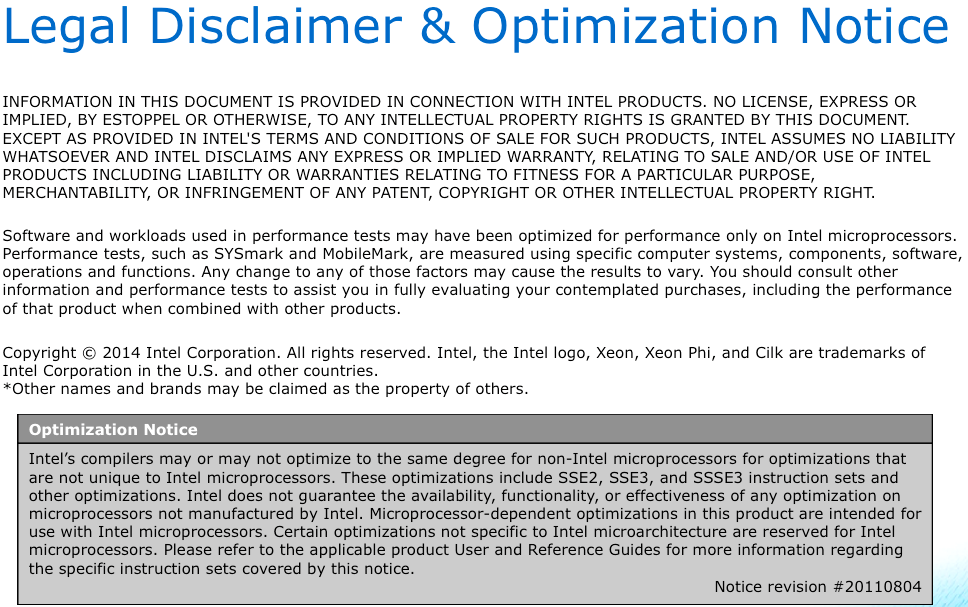
\includegraphics[scale=0.33,angle=0]{intel-legal} \
\end{frame}

\begin{frame}{Extreme Scalability Group Disclaimer}
    \begin{itemize}
        \item I work in Intel Labs and therefore don't know anything about Intel products.
        \item I work for Intel, but I am not an official spokesman for Intel.
              Hence anything I say are my words, not Intel's.
              Furthermore, I do not speak for my collaborators,
              whether they be inside or outside Intel.
        \item You may or may not be able to reproduce any performance numbers I report.
        \item Performance numbers for non-Intel platforms were obtained by non-Intel people.
        \item Hanlon's Razor.
    \end{itemize}
\end{frame}

\begin{frame}{Abstract (for posterity)}
    The MPI-3 standard provides a portable interface to interprocess 
    shared-memory through the RMA functionality. This allow applications 
    to leverage shared-memory programming within a strictly MPI paradigm, 
    which mitigates some of the challenges of MPI+X programming using 
    threads associated with shared-by-default behavior and race conditions, 
    NUMA and Amdahl's law. I will describe the MPI shared-memory capability 
    and how it might be targeted by existing multithreaded libraries.
\end{frame}

\begin{frame}{Quiz} \Large
    What is MPI? \\
    (A) A bulky, bulk-synchronous model. \\
    (B) The programing model based upon Send-Recv. \\
    (C) An explicit, CSP-like, private-address-space programming model. \\
    (D) An industry-standard runtime API encapsulating
        1-, 2- and $N$-sided blocking and nonblocking communication
        and a whole bunch of utility functions for library development. 
\end{frame}

\begin{frame}{The MPI You Know}
    \begin{tt}
        MPI\_Init(..); \\
        MPI\_Comm\_size(..); MPI\_Comm\_rank(..); \\
        MPI\_Barrier(..); MPI\_Bcast(..); \\
        MPI\_Reduce(..); MPI\_Allreduce(..); \\
        MPI\_Gather(..); MPI\_Allgather(..); \\
        MPI\_Scatter(..); MPI\_Alltoall(..); \\
        MPI\_Reduce\_scatter(..); MPI\_Reduce\_scatter\_block(..); \\
        MPI\_Send(..); MPI\_Recv(..); /* [b,nb] x [r,s,b] */ \\
        \ldots \\
        MPI\_Finalize();
    \end{tt}
\end{frame}

\begin{frame}{The MPI You Don't 1}
    \begin{tt}
        MPI\_Ibarrier(..); MPI\_Ibcast(..); \\
        MPI\_Ireduce(..); MPI\_Iallreduce(..); \\
        MPI\_Igather(..); MPI\_Iallgather(..); \\
        MPI\_Iscatter(..); MPI\_Ialltoall(..); \\
        MPI\_Ireduce\_scatter(..); MPI\_Ireduce\_scatter\_block(..); \\
    \end{tt}
    \vskip2ex
    Go forth a write bulk-asynchronous code!
\end{frame}

\begin{frame}{The MPI You Don't 2}
    \begin{tt}
        MPI\_Dist\_graph\_create\_adjacent(..); \\
        MPI\_Neighborhood\_allgather(..); \\
        MPI\_Neighborhood\_allgatherv(..); \\
        MPI\_Neighborhood\_alltoall(..); \\
    \end{tt}
    \vskip2ex
    Virtual topologies corresponding to algorithmic topology;
    additional semantic information enables MPI to optimize.
\end{frame}

\begin{frame}{The MPI You Don't 3}
    \begin{tt}
        Win\_create(..); Win\_allocate(..); \\
        Win\_allocate\_shared(..); Win\_shared\_query(..); \\
        Win\_create\_dynamic(..); Win\_attach(..); Win\_detach(..); \\
        Put(..); Get(..); Accumulate(..); \\
        Fetch\_and\_op(..); Compare\_and\_swap(..); \\
        Win\_lock(..); Win\_lock\_all(..); \\
        Win\_flush(\_local)(\_all)(..); Win\_sync(..); \\
        \ldots
    \end{tt}
    \vskip2ex
    MPI-3 is a superset of ARMCI and OpenSHMEM\ldots
    \vskip2ex
    \href{http://wiki.mpich.org/armci-mpi/}{http://wiki.mpich.org/armci-mpi/} \\
    \href{https://github.com/jeffhammond/oshmpi/}{https://github.com/jeffhammond/oshmpi/}
\end{frame}

\begin{frame}{Shared Memory implementations}
    Historically, SysV shared memory used, but painfully.
    \vskip1ex
    POSIX shared memory good, but Windows, BGQ, BSD/Mach\ldots
    \vskip1ex
    In HPC, we have XPMEM (Cray and SGI).
    \vskip1ex
    MPI processes can be threads, in which case, all is shared.
    \vskip1ex
    The purpose of MPI is to standardize best practice!
\end{frame}

\begin{frame}{MPI-3 Shared Memory}\Large
    Limitations: \\
    \begin{itemize}
        \item Only defined for cache-coherent systems (WIN\_MODEL=UNIFIED).
        \item Allocated collectively.
        \item Memory allocated contiguously \textit{by default}.
    \end{itemize}
    Features: \\
    \begin{itemize}
        \item Works together with RMA ops (e.g. atomics).
        \item Noncontiguous allocation upon request (hint).
    \end{itemize}
\end{frame}

\begin{frame}{Why should you use this?}\LARGE
    Shared memory programming is hard!!!! 
\end{frame}

\begin{frame}{} \LARGE
  \begin{center}
      \textbf{Challenges with MPI+X}
  \end{center}
\end{frame}

\begin{frame}[fragile]{The future is MPI+X}
\begin{itemize}
	\item MPI+OpenMP is too often fork-join.
	\item Pthreads scare people; can't be used from Fortran (easily).
	\item TBB and Cilk come from Intel (FYI: TBB now runs on BGQ).
	\item OpenCL is an eye chart and has no abstraction for performance variability.
	\item CUDA is an X for only one type of hardware (ignoring Ocelot).
\end{itemize}
Never confuse portability with portable performance!
\end{frame}

\begin{frame}{Using MPI+OpenMP effectively} \large 
\begin{itemize}
	\item Private data should behave like MPI but with load-store for comm.
	\item Shared data leads to cache reuse but also false sharing.
	\item NUMA is going to eat you alive.  BG is a rare exception.
	\item OpenMP offers little to no solution for NUMA.
	\item If you do everything else right, Amdahl is going to get you.
\end{itemize}
Intranode Amdahl and NUMA are giving OpenMP a bad name;
fully rewritten hybrid codes that exploit affinity behave very different
from MPI codes evolved into MPI+OpenMP codes.
\end{frame}

\begin{frame}{Fork-Join vs. Parallel-Serialize}
  \begin{center}
    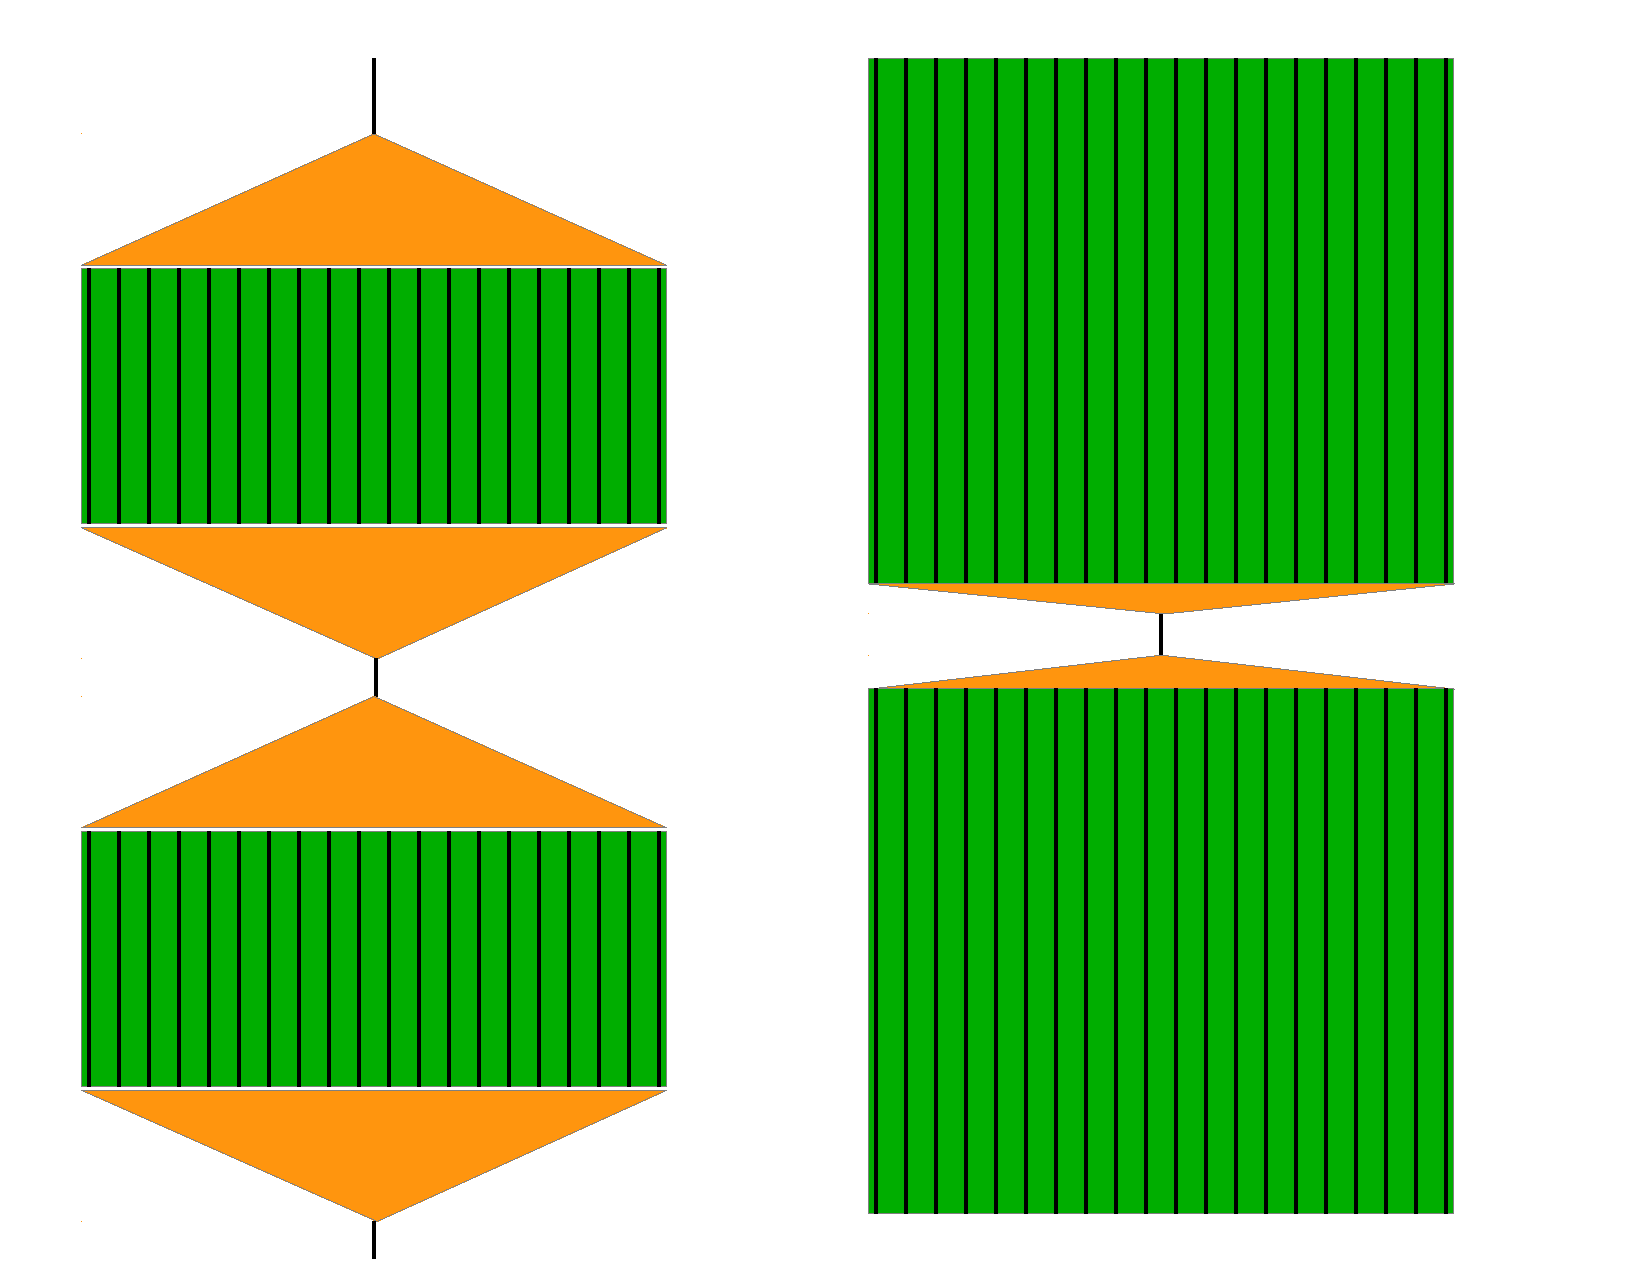
\includegraphics[scale=0.3,angle=0]{ForkJoin.pdf}
  \end{center}
\end{frame}

\begin{frame}{Fork-Join vs. Parallel-Serialize}
  \begin{columns}[T]
    \begin{column}{0.5 \linewidth}
      \begin{tt}
       \color{black}
       \#pragma omp parallel       \\
       \{ \\
       \color{green}
       /* thread-safe */      \\
       \vskip1ex
       \color{black}
       \#pragma omp single         \\
       \color{red}
       /* thread-unsafe */    \\
       \vskip1ex
       \color{black}
       \#pragma omp parallel for   \\
       \color{green}
       /* threaded loops */ \\
       \vskip1ex
       \color{black}
       \#pragma omp sections       \\
       {\color{green}
       /* threaded work */}  \\
       \}     \\
      \end{tt}
    \end{column}
    \begin{column}{0.5 \linewidth}
      \begin{tt}
       {\color{red} /* thread-unsafe */ }  \\
       \vskip1ex
       \color{black}
       \#pragma omp parallel for \\
       \{ \\
       {\color{green} /* threaded loops */} \\
       \} \\
       \vskip1ex
       {\color{red} /* thread-unsafe */ }  \\
       \vskip1ex
       \color{black}
       \#pragma omp parallel for \\
       \{ \\
       {\color{green} /* threaded loops */ } \\
       \} \\
       \vskip1ex
       \color{red}
       /* thread-unsafe work */  \\
      \end{tt}
    \end{column}
  \end{columns}
\end{frame}

\begin{frame}[fragile]{NUMA}
See \texttt{./src/omp/numa.c}
\begin{verbatim}
> for n in 1e6 1e7 1e8 1e9 ; do ./numa.x $n ; done
n = 1000000    a: 0.009927 b: 0.009947 
n = 10000000   a: 0.018938 b: 0.011763 
n = 100000000  a: 0.123872 b: 0.072453 
n = 1000000000 a: 0.915020 b: 0.811122 
\end{verbatim}
The first-order effect requires a multi-socket system so you will not see this on your laptop.
\vskip1ex
For more complicated data access patterns, you may see this even with parallel initialization.  
In this case, consider (1) hiding latency, (2) not being bandwidth bound, and (3) task parallelism.
\end{frame}

\begin{frame}{MPI+Y} \large 
\begin{itemize}
  \item If you use OpenMP libraries built with multiple compilers, you may get multiple thread pools.
  \item OpenMP, TBB, etc. all use Pthreads.  So do many apps and libraries.  Oversubscribe much?
  \item \texttt{MPI\_THREAD\_MULTIPLE} adds overhead; some apps use their own mutex 
  but internal mutexes are invisible to other MPI clients.
\end{itemize}
The stark reality is that general MPI+Y -- i.e. MPI+X for X$\ne$OpenMP -- is heavily dependent
upon an MPI implementation that is designed to be used in a truly multithreaded way.
Today, only Blue Gene/Q as this.
\vskip1ex
{\small Based on \url{https://www.ieeetcsc.org/activities/blog/challenges_for_interoperability_of_runtime_systems_in_scientific_applications} }
\end{frame}





\begin{frame}
\end{frame}

\begin{frame}
\end{frame}

\begin{frame}
\end{frame}

\begin{frame}
\end{frame}

\begin{frame}
\end{frame}

\begin{frame}
\end{frame}

\end{document}
